%%%%%%%%%%%%%%%%%%%%%%%%%%%%%%%%%%%%%%%%%%%%%%%%%%%%%%%%%%%%%%%%%%%%%%
% jckspaper.tex --  LaTeX2e-based template for submissions to National Speleological Society
% Journal Of Cave and Karst Studies
%
% Template developed by Malcolm Field, JCKS.
% Email questions to field.malcolm@epa.gov.
%
%
%%%%%%%%%%%%%%%%%%%%%%%%%%%%%%%%%%%%%%%%%%%%%%%%%%%%%%%%%%%%%%%%
%%%%%%%%%%%%%%%%%%%%%%%%%%%%%%%%%%%%%%%%%%%%%%%%%%%%%%%%%%%%%%%%
%																															 %
%				USE THIS TEMPLATE, JCKS1COL.STY, AND JCKS.BST				 %
%			        OR YOUR TEX FILES WILL NOT BE USED				  		 %
%																															 %
%%%%%%%%%%%%%%%%%%%%%%%%%%%%%%%%%%%%%%%%%%%%%%%%%%%%%%%%%%%%%%%%
%%%%%%%%%%%%%%%%%%%%%%%%%%%%%%%%%%%%%%%%%%%%%%%%%%%%%%%%%%%%%%%%
%
% Main template file for LaTeX for Journal of Cave and Karst Studies
%
%%%%%%%%%%%%%%%%%%%%%%%%%%%%%%%%%%%%%%%%%%%%%%%%%%%%%%%%%%%%%%%%%%%%%%%%%%%%
% This sample file is for articles formatted with LaTeX2e,
% Modified November 2010
%
% This template is set up logically, with commands and instructions
% given in the order necessary to produce a final output that will
% satisfy JCKS requirements.
%
% PLEASE DO NOT USE YOUR OWN MACROS
%
% All questions should be e-mailed to field.malcolm@epa.gov.
%%%%%%%%%%%%%%%%%%%%%%%%%%%%%%%%%%%%%%%%%%%%%%%%%%%%%%%%%%%%%%%%%%%%%%%%%%%%
%
% ARTICLE MODE
%
% Preamble for LaTeX for Journal of Cave and Karst Studies
% Last edit: November 18, 2010
%%%%%%%%%%%%%%%%%%%%%%%%%%%%%%%%%%%%%%%%%%%%%%%%%%%%%%%%%%%%%%%%%%%%%
% PREAMBLE

% % The \cite command functions used with the Natbib package is as follows:
 %   \citet{key} ==>>                Jones et al. (1990)
 %   \citet*{key} ==>>               Jones, Baker, and Smith (1990)
 %   \citep{key} ==>>                (Jones et al., 1990)
 %   \citep*{key} ==>>               (Jones, Baker, and Smith, 1990)
 %   \citep[chap. 2]{key} ==>>       (Jones et al., 1990, chap. 2)
 %   \citep[e.g.][]{key} ==>>        (e.g. Jones et al., 1990)
 %   \citep[e.g.][p. 32]{key} ==>>   (e.g. Jones et al., p. 32)
 %   \citeauthor{key} ==>>           Jones et al.
 %   \citeauthor*{key} ==>>          Jones, Baker, and Smith
 %   \citeyear{key} ==>>             1990

%%%%%%%%%%%%%%%%%%%%%%%%%%%%%%%%%%%%%%%%%%%%%%%%%%%%%%%%%%%%%%%%%%%%%
%
% The following two commands will generate a PDF that follows all the requirements for submission
% and peer review.  Uncomment these commands to generate this output (and comment out the two lines below.)
%
% DOUBLE SPACE VERSION FOR SUBMISSION TO THE JOURNAL OF CAVE AND KARST STUDIES
\documentclass[12pt]{article}
\usepackage{jcks1col}
%
% The following two commands will generate a single space, double column paper that closely
% matches an JCKS journal page.  Uncomment these commands to generate this output (and comment
% out the two lines above. FOR AUTHOR USE ONLY. PAPERS SUBMITTED IN THIS FORMAT WILL BE RETURNED
% TO THE AUTHOR for submission with the correct formatting.
%
% TWO COLUMN JOURNAL PAGE LAYOUT FOR AUTHOR USE ONLY
%\documentclass[10pt]{article}
%\usepackage{jcks2col}
%
%%%%%%%%%%%%%%%%%%%%%%%%%%%%%%%%%%%%%%%%%%%%%%%%%%%%%%%%%%%%%%%%%%%%%%%%%%%%%%%%%
% ABSTRACT
%
% Enter your Abstract between main enclosing parentheses here
%%%%%%%%%%%%%%%%%%%%%%%%%%%%%%%%%%%%%%%%%%%%%%%%%%%%%%%%%%%%%%%%%%%%%%%%%%%%%%%%%
\newcommand{\myabstract}{Enter the text of your abstract here. This is a sample \textit{Journal of Cave and Karst Studies} (JCKS) \LaTeX\ template.  This document provides authors with both a \LaTeX\ template and basic JCKS formatting guidelines to be used when writing a paper.  Authors should refer to the file jckspaper.tex to review the actual \LaTeX\ code used to create this document.  The jckspaper.tex (or blank\_template.tex) file can then be modified by authors for their own manuscript. The abstract should be no longer than 250 words in length.  The abstract should not contain any mathematical expressions, should not include any footnotes or citations, and should not contain first-person sentence structure.}

%
%%%%%%%%%%%%%%%%%%%%%%%%%%%%%%%%%%%%%%%%%%%%%%%%%%%%%%%%%%%%%%%%%%%%%%%%%%%%%%%%%
% KEYWORDS
%
% Enter your Keywords between main enclosing parentheses here
%%%%%%%%%%%%%%%%%%%%%%%%%%%%%%%%%%%%%%%%%%%%%%%%%%%%%%%%%%%%%%%%%%%%%%%%%%%%%%%%%
\newcommand{\mykeywords}{Enter no more than six keywords separated by commas here.}

%
%%%%%%%%%%%%%%%%%%%%%%%%%%%%%%%%%%%%%%%%%%%%%%%%%%%%%%%%%%%%%%%%%%%%%%%%%%%%%%%%%
% DOCUMENT START
%
% Begin entering your document text below (after \begin{document} command)
%%%%%%%%%%%%%%%%%%%%%%%%%%%%%%%%%%%%%%%%%%%%%%%%%%%%%%%%%%%%%%%%%%%%%%%%%%%%%%%%%
\begin{document}
%
%%%%%%%%%%%%%%%%%%%%%%%%%%%%%%%%%%%%%%%%%%%%%%%%%%%%%%%%%%%%%%%%%%%%%
% TITLE
%
% Enter your TITLE here
%%%%%%%%%%%%%%%%%%%%%%%%%%%%%%%%%%%%%%%%%%%%%%%%%%%%%%%%%%%%%%%%%%%%%
\title{\textbf{\large{A Sample \textit{Journal of Cave and Karst Studies} \LaTeX\ Document}}}
%
% Author names, with corresponding author information.
% Use \\ as necessary to start a new line for author address information
% [Update and move the \thanks{...} block as appropriate.]
%

\author{Malcolm S.\ Field\protect\thanks{\textit{Corresponding Author}} \\
Office of Research and Development, U.S.\ Environmental Protection Agency \\
1200 Pennsylvania Ave., NW, Washington, DC 20460-0001, USA \\
field.malcolm@epa.gov
\and
\centerline{Second Author} \\ % Add additional authors, different institution
Affiliation, City, State/Province, Postal Code, Country \\
e-mail address}
%
% The following block of code will handle the formatting of the title page depending on whether
% we are formatting a double column (dc) author draft or a single column paper for submission.
% AUTHORS SHOULD SKIP OVER THIS... There is nothing to do in this section of code.
%
\ifthenelse{\boolean{dc}}
{
\twocolumn[
\begin{@twocolumnfalse}
    \jckstitle

% Start Abstract (Enter your Abstract above.  Do not enter any text here)
    \begin{center}
        \begin{minipage}{13.0cm}
            \begin{abstract}
                \myabstract \\     % Linebreak here provides a space between abstract and keywords
            \end{abstract}
            \begin{keywords}
                \mykeywords
            \end{keywords}
            \begin{center}
                \rule{38mm}{0.2mm}
            \end{center}
        \end{minipage}
    \end{center}
\end{@twocolumnfalse}
]
}
{
\jckstitle
\begin{abstract}
    \myabstract
\end{abstract}
\begin{keywords}
    \mykeywords
\end{keywords}
\newpage
}

% Automatically begin line numbering here for manuscript, but not preprints.
% Note that line numbering is required for submission but not for preprints.
\ifthenelse{\boolean{dc}}
{}
{\linenumbers}

%%%%%%%%%%%%%%%%%%%%%%%%%%%%%%%%%%%%%%%%%%%%%%%%%%%%%%%%%%%%%%%%%%%%%
% MAIN BODY OF PAPER
%%%%%%%%%%%%%%%%%%%%%%%%%%%%%%%%%%%%%%%%%%%%%%%%%%%%%%%%%%%%%%%%%%%%%
%
\section{Introduction}
This document will provide authors with the basic \textit{Journal of Cave and Karst Studies} (JCKS) formatting guidelines.  This document was created using \LaTeX\, and demonstrates how to use the \LaTeX\ template when submitting a manuscript to the JCKS.  The following sections will outline the guidelines and formatting for text, math, figures, and tables while using \LaTeX\/.  A more thorough review of all manuscript requirements can be found in the JCKS Authors' Guide (available online at \url{http://www.caves.org/pub/journal/Guide.htm}).

An attempt to compile jckspaper.tex should be made before using the template.  The files have been tested on a Windows XP using WinEdt using MiKTeX.  Other distributions of Linux/Unix, Windows, and \LaTeX\ may be acceptable.  Feedback and questions should be sent to \url{field.malcolm@epa.gov}.

Authors may use the empty template blank\_template.tex to begin their paper.  A valuable source of \LaTeX\ information are the \textit{Tex Frequently Asked Questions} available at numerous Web sites (available online at \url{faq.tug.org}).

\section{Formatting Text and Sections}
The text should be divided into sections, each with a separate heading and consecutive numbering.  Each section heading should be placed on a separate line using the appropriate \LaTeX\ commands.  For more detailed information on different sections and their formatting see the Authors' Guide.

\subsection{Secondary Headings}
Secondary headings are formatted using the $\backslash$subsection\{\} command for secondary sections.

\subsubsection{Tertiary Headings}
Tertiary headings are formatted using the $\backslash$subsubsection\{\} command.

\paragraph{Quaternary Headings}
Quaternary headings are formatted using the $\backslash$paragraph\{\} command.

\section{JCKS Web Site}
After completing your manuscript, then load it, and any style files (e.g., jcks1col.sty), figure files, references file, and if created separately, any table files to the \url{http://www.edmgr.com/jcks/} system.  Note that each style file called in your manuscript using the $\backslash$usepackage\{\} must be uploaded.  Also note that some style files (e.g., siunitx, breakurl) may not work with Editorial Manager, which the JCKS web site is built on.

\section{Style Files}
Several style file packages are automatically loaded when the style file, jcks1col.sty (or jcks2col.sty), is loaded as $\backslash$usepackage\{jcks1col\} at the beginning of a manuscript file (see the first line after ``$\backslash$documentclass[12pt]\{article\}'' near the top of this file.  If jcks1col.sty is or jcks2col.sty is loaded using the $\backslash$usepackage command in a manuscript (see top of this file) then several style files will automatically be loaded and do not require specifying in \url{http://www.edmgr.com/jcks/}.  These style files are:

% Use "itemize," "list," or "trivlist" for simple listing of items.  Use "description" or "enumerate" environments for
% more detailed lists.
\begin{itemize}
\item geometry
\item natbib
\item url
\item xcolor
\item fancyhdr
\item ccaption
\item booktabs
\item threeparttable
\item warpcol
\item icomma
\item amsmath, amsfonts, amssymb, bm
\item indentfirst
\item lineno
\item ifthen
\item endfloat
\item ragged2e
\item titlesec
\end{itemize}
A brief description of each listed style file can be found in the required style files, jcks1col.sty and jcks2col.sty.  More comprehensive descriptions of each may be found at \url{www.ctan.org} and up-to-date textbooks on \LaTeX.

\section{Citations}
Citations to standard references in text should consist of the name of the author and the year of publication, for example, \citet{mohammadifield09} or \citep{fieldli10} using the appropriate $\backslash$citet or $\backslash$citep commands, respectively.  A variety of citation formats can be used with the natbib package.  Refer to documentation on the natbib package for more information on the basic citation commands.  References should be entered in the references.bib file located in the bibliography subdirectory.  For a thorough discussion of how to enter references into the references.bib database file following JCKS style please refer to the jcks\_references.pdf document included in this package.  Basic citation commands are:

% Use tabbing or tabular environments when appropriate
\begin{tabbing}
\07. \= $\backslash$citep[e.g.,][p. 32]\{key\} \= $\Rightarrow$ \= (e.g., Jones et al., p. 32) \kill
\01. \> $\backslash$citet\{key\}               \> $\Rightarrow$ \> Jones et al. (1990) \\
\02. \> $\backslash$citet*\{key\}              \> $\Rightarrow$ \> Jones, Baker, and Smith (1990) \\
\03. \> $\backslash$citep\{key\}               \> $\Rightarrow$ \> (Jones et al., 1990) \\
\04. \> $\backslash$citep*\{key\}              \> $\Rightarrow$ \> (Jones, Baker, and Smith, 1990) \\
\05. \> $\backslash$citep[chap. 2]\{key\}      \> $\Rightarrow$ \> (Jones et al., 1990, chap. 2) \\
\06. \> $\backslash$citep[e.g.,][]\{key\}      \> $\Rightarrow$ \> (e.g., Jones et al., 1990) \\
\07. \> $\backslash$citep[e.g.,][p. 32]\{key\} \> $\Rightarrow$ \> (e.g., Jones et al., p. 32) \\
\08. \> $\backslash$citeauthor\{key\}          \> $\Rightarrow$ \> Jones et al. \\
\09. \> $\backslash$citeauthor*\{key\}         \> $\Rightarrow$ \> Jones, Baker, and Smith \\
 10. \> $\backslash$citeyear\{key\}            \> $\Rightarrow$ \> 1990 \\
\end{tabbing}
See commented section at beginning of this template for actual form that the citations commands may take.  Also, note that numbers 2, 4, 9, and 10 are not allowed in manuscripts to be published in JCKS.  Lastly, note usage of the phantom character ``$\backslash 0$'' in front of numbers 1--9 to facilitate alignment with number 10.

\section{Formatting Math}
The following sections will outline the basic formatting rules for mathematical symbols and units.  In addition, a review of the jckspaper.tex file will show how this is done with the use of \LaTeX\ commands.  The JCKS template provides the American Mathematical Society math, font, symbol, and boldface packages for use in math mode.

\subsection{Mathematical Symbols}
Symbols must be of the same font style both in text discussion and in displayed equations or terms (and figures should be prepared to match).  Scalar single character symbols are set italic, Greek, or script.  Examples are $u$, $L$ [note that $\upsilon$ (Greek upsilon) is used instead of \textit{v} (italic ``vee'') to avoid confusion with  $\nu$ (Greek nu) often used for viscosity; this is handled automatically when in \LaTeX\ math mode], $w$, $x$, $y$, $z$, $f$, $g$, $r$, indices such as $i$ or $j$, and constants such as $C_D$, $k$, or $K$.  Multiple character scalar variables, abbreviations, nondimensional numbers, and acronyms for variables are set regular nonitalic: $\mathrm{LWC}$, $\mathrm{Re}$, $\mathrm{Ro}$, $\mathrm{BT}$, $\mathrm{abs}$, $\mathrm{obs}$, $\mathrm{max}$, $\mathrm{min}$, $\mathrm{Re}$/$\mathrm{Im}$ (real/imaginary), etc.  For vectors, use boldface nonitalic Times Roman as in $\mathbf{V}$, $\mathbf{v}$, or $\mathbf{x}$, and $\mathbf{i}$, $\mathbf{j}$, and $\mathbf{k}$ unit vectors. Do not use the \LaTeX\ $\backslash$vec command to denote vectors.  For matrix notation use nonitalic boldface Arial (or Sans Serif) font as in $\bm{\mathsf{A}}$, $\bm{\mathsf{B}}$, or $\bm{\mathsf{M}}$.  All mathematical operator abbreviations/acronyms are set lowercase regular Roman font, except $O$ (on the order of): $\sin$, $\cos$, $\tan$, $\tanh$, $\mathrm{cov}$, $\Pr$ (for probability; note same as Prandtl number), $\mathrm{const}$ (for constant), $\mathrm{c.c.}$ (complex conjugate).

\subsection{Units}
Units are always set on a single line with a tilde (or, less preferably, a space) separating the denominator, which is set with a superscript $-1$, $-2$, and so on, rather than using a slash for ``per.''  Examples are g kg$^{-1}$ , m$^2$~s$^{-1}$, W~m$^{-2}$, g~m$^{-3}$, and m~s$^{-1}$ (note that ms$^{-1}$ is the unit for ``per millisecond'').  Note that the style file, SIunits, will automatically set units properly as will siunitx (but siunitx will not work with PeerTrack so siunitx cannot be used).

\subsection{Equations}
Brief equations or terms set inline in text must be set as a single line expression because page proofs are not double spaced, for example, $\rho^{-1}p/x$ or $(1/{\rho})p/x$  or $(a-b)/(c+d)$; that is, use a superscript $-1$ for the denominator.  In case of a more complicated term or equation, it should be set as an unnumbered display equation,
such as the binomial equation
\begin{displaymath}
(x+a)^n = \sum^{n}_{k=0} \binom{n}{k} x^k a^{n-k}.
\end{displaymath}
Otherwise, numbered display equations can be entered using the appropriate $\backslash$begin\{equation\} command, such as the arithmetic mean and standard deviation given by, respectively
\begin{equation}
\overline{x}_b = \frac{1}{n}\sum_{i=1}^n x_i,                                              \label{eq:amean}
\end{equation}
and
\begin{equation}
s_b = \sqrt{\frac{1}{n-1}\sum_{i=1}^n (x_i - \overline{x}_b)^2}.                            \label{eq:sdev}
\end{equation}

Note the punctuation in the three equations shown.  Lists of equations are punctuated as written English, and commas, semicolons, and periods that are placed where appropriate.  Conjunctions such as ``and,'' ``while,'' ``when,'' or ``for'' are also typically placed before the final element in a mathematical phrase, as befits the intended mathematical meaning.

Overly long equations that may extend across the with of a single-column page may run over the text when the accepted manuscript is printed in the standard two-column format.  Therefore, very long equations should be split into multiple rows to facilitate proper printing.  For example,
\begin{equation}
    \begin{split}
        C_{\text{IVP}}(z,t) &= \int_0^L C_{\text{I}}(\zeta)\biggl\{\frac{1}{\sqrt{4 \pi D t}}\exp\biggl[\frac{-(z-W t - \zeta)^2}{4 D t}\biggr] \\
        &- \int_0^t \frac{1}{\sqrt{4 \pi D \tau}}\exp\biggl[\frac{-(W t + \zeta)^2}{4 D \tau}\biggr]\frac{z}{4 \pi D(t - \tau)^3} \\
        &\times \exp\biggl[\frac{-[z-W(t - \tau)]^2}{4 D(t - \tau)}\biggr] d\tau \biggr\} d\zeta.
    \end{split}
    \label{eq:ivsolu}
\end{equation}

\section{Figures and Tables}

\subsection{Figures}
Detailed information about figures can be found both in the Authors' Guide and through links on the JCKS Author Upload Web page (available online at \url{http://www.ametsoc.org/au_upload/index.cfm}).  The insertion of a sample figure (Fig.~\ref{fig:figure1}) and caption is shown above.  Standard figure sizes are 19 (one column), 27, 30, 33 (two columns), 36, and 39 picas.  Authors should attempt to size their figures appropriately.  At this time our press can accept only PS, EPS, and TIFF figures.  Because pdfTeX does not support the use of either of these figure types authors should not attempt to build their PDF file using this driver.  The dvips driver does support the use of EPS files, but not TIFF files.  Therefore, authors should use EPS figure files when using this template.

%%%%%%%%%%%%%%%%%%%%%%%%%%%%%%%%%%%%%%%%%%%%%%%%%%%%%%%%%%%%%%%%%%%%%
% FIGURES
%%%%%%%%%%%%%%%%%%%%%%%%%%%%%%%%%%%%%%%%%%%%%%%%%%%%%%%%%%%%%%%%%%%%%
\begin{figure}
\begin{center}
%\noindent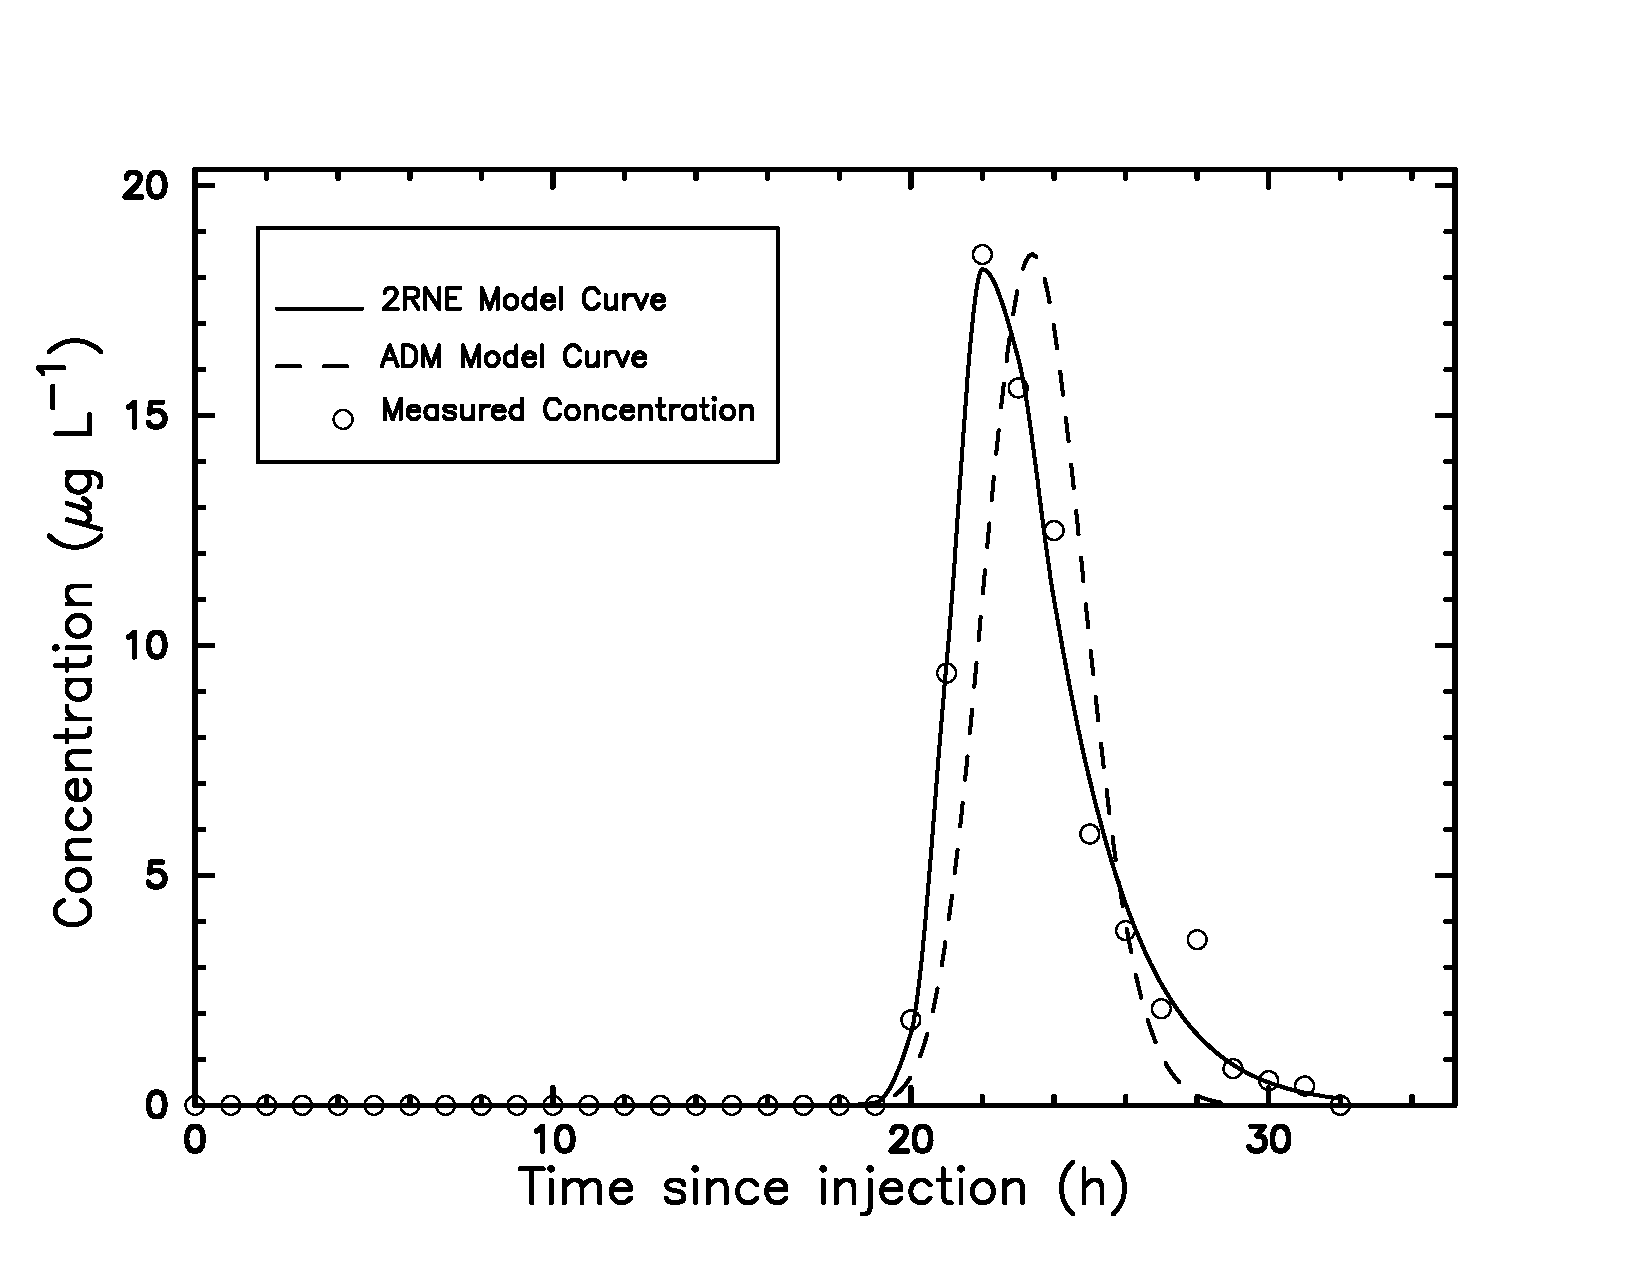
\includegraphics[width=23pc,angle=0]{Lost} \\ %%%%%%%%%% YOU MUST COMMENT OUT THIS LINE WHEN SUBMITTING YOUR MANUSCRIPT %%%%%%%
\caption{Enter the caption for your figure here.  Repeat as necessary for each of your figures.  Create a figures directory and place all figures in that directory.  Figure from \citet{fieldli10}.}
\label{fig:figure1}
\end{center}
\end{figure}

\subsection{Tables}
Each table must be numbered, provided with a caption, and mentioned specifically in the text.  Each table should appear on a separate page with an explanatory caption typed above the table on the same page.  All tables should be attached at the end of the manuscript, following the figure legends.  See \url{http://www.caves.org/pub/journal/PDF/Tables.pdf} for more information on the proper preparation of tables.  See below for the formatting of a sample table (Table~\ref{tab:table1}).  Please note that the first column of Table~\ref{tab:table1} was formatted using ``P{1.3},'' which is provided when using the warpcol package and allows formatting on the decimal point.  Alternatively, this could have been achieved using the dcolumn package (which would need to be added to this file) or by means of the phantom character ``$\backslash$0.''

%%%%%%%%%%%%%%%%%%%%%%%%%%%%%%%%%%%%%%%%%%%%%%%%%%%%%%%%%%%%%%%%%%%%%
% TABLES
%%%%%%%%%%%%%%%%%%%%%%%%%%%%%%%%%%%%%%%%%%%%%%%%%%%%%%%%%%%%%%%%%%%%%
% One column table
\begin{table}
\begin{center}
\begin{threeparttable}
\caption{Increasing and then decreasing inflow rates used to model sinkhole drainage.}
\begin{tabular}{P{1.3} c c c c}
\toprule
\multicolumn{1}{r}{} &
\multicolumn{4}{c}{Inflow Rates, $Q_i$, m$^3$~s$^{-1}$} \\
\cmidrule{2-5}
%
\multicolumn{1}{l}{Time\tnote{a}, s} &
\multicolumn{1}{r}{$Q_1 \gg q$} &
\multicolumn{1}{r}{$Q_2 > q$} &
\multicolumn{1}{r}{$Q_3 = q$} &
\multicolumn{1}{r}{$Q_4 \ll q$} \\
\midrule
%
0.    & 0.240 & 0.190 & 0.147 & 0.020 \\
400.  & 0.246 & 0.193 & 0.149 & 0.025 \\
800.  & 0.250 & 0.196 & 0.150 & 0.026 \\
1200. & 0.254 & 0.199 & 0.152 & 0.032 \\
1600. & 0.258 & 0.202 & 0.154 & 0.048 \\
2000. & 0.262 & 0.205 & 0.155 & 0.062 \\
2400. & 0.250 & 0.200 & 0.153 & 0.059 \\
2800. & 0.237 & 0.194 & 0.149 & 0.057 \\
3200. & 0.229 & 0.189 & 0.146 & 0.056 \\
3600. & 0.221 & 0.185 & 0.143 & 0.052 \\
4000. & 0.213 & 0.180 & 0.140 & 0.045 \\
\bottomrule
\end{tabular}
\label{tab:table1}
\begin{tablenotes}
\footnotesize
\item[a] Zero time represents initial inflow rates.
\item[] Note decimal alignment of first column using special command, ``P{1.3}'', based on included package, warpcol.sty.
\item[] Note that three dots may be entered in any location for no data using the ``$\backslash$nodata'' command.
\normalsize
\end{tablenotes}
\end{threeparttable}
\end{center}
\end{table}

%
%%%%%%%%%%%%%%%%%%%%%%%%%%%%%%%%%%%%%%%%%%%%%%%%%%%%%%%%%%%%%%%%%%%%%
% ACKNOWLEDGMENTS
%%%%%%%%%%%%%%%%%%%%%%%%%%%%%%%%%%%%%%%%%%%%%%%%%%%%%%%%%%%%%%%%%%%%%
%
\section{Acknowledgements}

Enter your acknowledgements here.  Keep acknowledgements as brief as possible (note correct spelling does not allow for an ``e'' between the ``g'' and ``m'').  In general, acknowledgements should only be directed to help in writing, research, or the providing of figures or photos.  Contribution of figures or photos should be acknowledge here rather than under the respective figure or photo as is often done in nonscientific publications (i.e., magazines).  Financial support (e.g., grant numbers) for the work done, or for an author, or for the laboratory where the work was performed is best acknowledged here rather than as footnotes to the title or to an author's name.  Contribution numbers (if the work has been published by the author's institution or organization) should be included on the title page, not in the acknowledgements.

%%%%%%%%%%%%%%%%%%%%%%%%%%%%%%%%%%%%%%%%%%%%%%%%%%%%%%%%%%%%%%%%%%%%%
% Notations
%%%%%%%%%%%%%%%%%%%%%%%%%%%%%%%%%%%%%%%%%%%%%%%%%%%%%%%%%%%%%%%%%%%%%
% Add Notations section to manuscript here (just before references).  Note form shown; $a_0$ is listed at the top line
% because it is the widest variable.  The widest variable defines the necessary width for all other variables defined in
% the Notations section.
\begin{notation}{$C_{\text{IVP}}$} % Enter your longest symbol inside the parentheses here
\item[$C_{\text{IVP}}$]          Concentration for initial value problem [M~L$^{-3}$]
\item[$D$]                       Longitudinal dispersion [L$^2$~T$^{-1}$]
\item[$t$]                       Time [T]
\end{notation}

%%%%%%%%%%%%%%%%%%%%%%%%%%%%%%%%%%%%%%%%%%%%%%%%%%%%%%%%%%%%%%%%%%%%%
% REFERENCES
%%%%%%%%%%%%%%%%%%%%%%%%%%%%%%%%%%%%%%%%%%%%%%%%%%%%%%%%%%%%%%%%%%%%%
% Create a bibliography directory and place your .bib file there.  You can either use BibTeX as was done here---Note that you must
% use JCKS.bst for your bibliography.  Alternatively you can enter your references using bibitem as is shown below, but commented out here.
%
\ifthenelse{\boolean{dc}}
{}
{\clearpage}
\bibliographystyle{jcks}
\bibliography{jcks_references}

%\begin{thebibliography}
%%
%\bibitem[{Field and {Guangquan Li}(2010)}]{fieldli10}
%Field, M.S., and {Guangquan Li}, 2010, Inversion for the input history of a dye
%  tracing experiment: Journal of Cave and Karst Studies, v.~73, no.~1, p.
%  16--20.
%
%\bibitem[{Mohammadi and Field(2009)}]{mohammadifield09}
%Mohammadi, Z., and Field, M.S., 2009, On the temporal behaviour of karst
%  aquifers, {Z}agros region, {I}ran: A geostatistical approach: Journal of Cave
%  and Karst Studies, v.~71, no.~3, p. 210--226.
%
%\end{thebibliography}

%%%%%%%%%%%%%%%%%%%%%%%%%%%%%%%%%%%%%%%%%%%%%%%%%%%%%%%%%%%%%%%%%%%%%
% APPENDICES
%%%%%%%%%%%%%%%%%%%%%%%%%%%%%%%%%%%%%%%%%%%%%%%%%%%%%%%%%%%%%%%%%%%%%
% Add appendices here if appendices are to be included in manuscript.
\ifthenelse{\boolean{dc}}
{}
{\clearpage}
\setcounter{equation}{0}% reset counter
\section{Appendix I}% Use \section{Appendix} and not \section{Appendix I} for only one appendix.
\section{Appendix Title Is Entered Here}
\subsection{Appendix Section}
The JCKS template allows authors to format an unlimited number of appendixes.  To format a single appendix, just create the appendix within the appropriate sectioning command. Otherwise, add the appropriate one-letter argument to the ``Appendix'' header (e.g., Appendix I, Appendix II, Appendix III, etc.) corresponding to the appropriate appendix.  The title of the appendix is then formatted using the $\backslash$section command as shown above (which also provides the code for centering).  The $\backslash$subsection, $\backslash$subsubection, and $\backslash$paragraph commands are used to create sections within the appendix.  Equations are automatically numbered appropriately for each appendix.  Here is an example of the first equation in Appendix I, automatically labeled as Equation~(\ref{eq:pde}),
\begin{equation}
\frac{\partial u}{\partial t} = \frac{1}{r}\frac{\partial}{\partial r}\biggl(r\frac{\partial u}{\partial r}\biggr) + \frac{1}{r^2}\frac{\partial^2 u}{\partial \theta^2} + \frac{\partial^2 u}{\partial z^2}.
\label{eq:pde}
\end{equation}

\ifthenelse{\boolean{dc}}
{}
{\clearpage}
\setcounter{equation}{0}% reset counter
\section{Appendix II}
\section{File structure of the JCKS \LaTeX\ Package}
\subsection{JCKS \LaTeX\ Files}
You will be provided with a tarred, zipped \LaTeX\ package containing eleven files: jckspaper.tex, blank\_template.tex, jcks1col.sty, jcks2col.sty, jckspaper.pdf, jckspaper2col.pdf, figure01.eps, jcks\_references.pdf, jcks.bst, database.bib, and references.bib.  Two subdirectories will be created when you unzip the package: figures and bibliography.  The figures directory will contain the sample figure file figure01.eps.  This directory should be used to store all your figure files.  The bibliography directory will contain the sample bibliography files database.bib and references.bib.  You should alter references.bib with your own bibliography information.  Refer to the jcks\_references.pdf file included in this package for information on how to properly populate the references.bib file. The files jcks1col.sty and jcks2col.sty are the two style files.  The file jcks1col.sty generates a PDF that follows all JCKS guidelines for submission and peer review.  The file jcks2col.sty can be used to generate a PDF that closely follows the layout of an JCKS journal page, including single spacing and two columns.  This journal style PDF is only for the author's personal use, and any papers submitted in this style will not be accepted.  Always use the jcks1col.sty when generating a PDF for submission to the JCKS. The file jcks.bst is the bibliography style file.  The file jckspaper.tex contains the \LaTeX\ code for this sample file.   The resulting PDF can be seen in either jckspaper.pdf or jckspaper2col.pdf, depending on the which style file is used. The file blank\_template.tex provides a basic blank template with some section headings for authors to more easily enter their manuscript into.

\ifthenelse{\boolean{dc}}
{}
{\clearpage}
\setcounter{equation}{0}% reset counter
\section{Appendix III}
\section{How to Compile the \LaTeX\ Files and Create a PDF}
\subsection{Compilation}
There are a variety of different methods and programs that will create a final PDF from your \LaTeX\ document.  Here, the basic commands for one method of creating a final PDF are presented. You can compile your \LaTeX\ files and build the dvi file with the following commands on a Linux-/Unix-based system:

%
%Use "enumeration" lists for numbered lists.
\begin{enumerate}
\item latex filename.tex (e.g., latex jckspaper.tex)
\item bibtex filename (e.g., bibtex jckspaper).  Note that the .tex extension is not included in the filename
\item latex filename.tex (e.g., latex jckspaper.tex)
\item latex filename.tex (e.g., latex jckspaper.tex).  This command is repeated twice to clean up any reference dependencies.
\end{enumerate}
This will create a dvi file (e.g., jckspaper.dvi).  You can view the dvi file using a dvi file viewer, such as xdvi, kdvi, or some similar program.  Your PDF will be created from the dvi file, so do not delete this file.

\subsection{Creating the PDF}
The final PDF can be created from the dvi file using the following two commands on a Linux-/Unix-based system:
\begin{itemize} % Use "itemize" lists for unnumbered lists, but bullets are not used.
\item[]{dvips filename.dvi -o filename.ps (e.g., dvips jckspaper.dvi -o   jckspaper.ps), which converts the dvi file to a postscript file that will be converted to the final PDF; and}
\item[]{ps2pdf14 filename.ps (e.g., ps2pdf14 jckspaper.ps), which creates the final PDF file (jckspaper.pdf).  The ``14'' at the end of the ps2pdf14 command will   generate a PDF compatible with Acrobat Reader, version 5 and later. It may be replaced with ps2pdf13 or ps2pdf, which will generate PDFs compatible with Acrobat Reader, version 4 or 3 and later,
  respectively.}
\end{itemize}
It is much easier to generate a *.dvi file or a *.pdf file directly on a Windows machine running WinEdt (shareware) and MiK\TeX (freeware) or similar packages.  The operations require nothing more than a click of the appropriate icons at the top of the screen.

\subsection{Other software}
There is a variety of software that can be used to edit .tex files and build a PDF.  The JCKS does not support \LaTeX\/-related WYSIWYG software, such as Scientific Workplace, or WYSIWYM software, such as LyX.  \TeX\ Live (available online at \url{http://www.tug.org/texlive/}) is recommended for users needing an up-to-date \LaTeX\ distribution with software that includes an editor and the ability to automatically generate a PDF.


\end{document}
%%%%%%%%%%%%%%%%%%%%%%%%%%%%%%%%%%%%%%%%%%%%%%%%%%%%%%%%%%%%%%%%%%%%%
% END OF TEMPLATE
%%%%%%%%%%%%%%%%%%%%%%%%%%%%%%%%%%%%%%%%%%%%%%%%%%%%%%%%%%%%%%%%%%%%%